\documentclass[a4paper,12pt]{article}
\usepackage{url}
\usepackage{graphicx}
\usepackage{amsmath}
\usepackage{geometry}
\usepackage{float}
\usepackage{tikz}
\usepackage{circuitikz}
\usepackage{booktabs}
\usepackage{algorithm}
\usepackage{algorithmic}
\usepackage{array}
\usepackage{hyperref}
\usepackage{listings}
\usepackage{xcolor}
\geometry{margin=1in}

\title{Scientific Calculator Using AVR-GCC}
\author{EE24BTECH11005: Credits EE24BTECH11001, EE24BTECH11002}
\date{\today}

\begin{document}

\maketitle

\section*{Introduction}
This project presents a scientific calculator built using the AtMega328p microcontroller with the avr-gcc framework. Instead of relying on standard libraries, an effort was made to implement mathematical functions using differential equations, staying true to the motto of the course. Special attention was given to creating a user-friendly interface with features like the ability to review and edit inputs, making the calculator both functional and easy to use.
\begin{figure}[h!]
  \begin{center}
    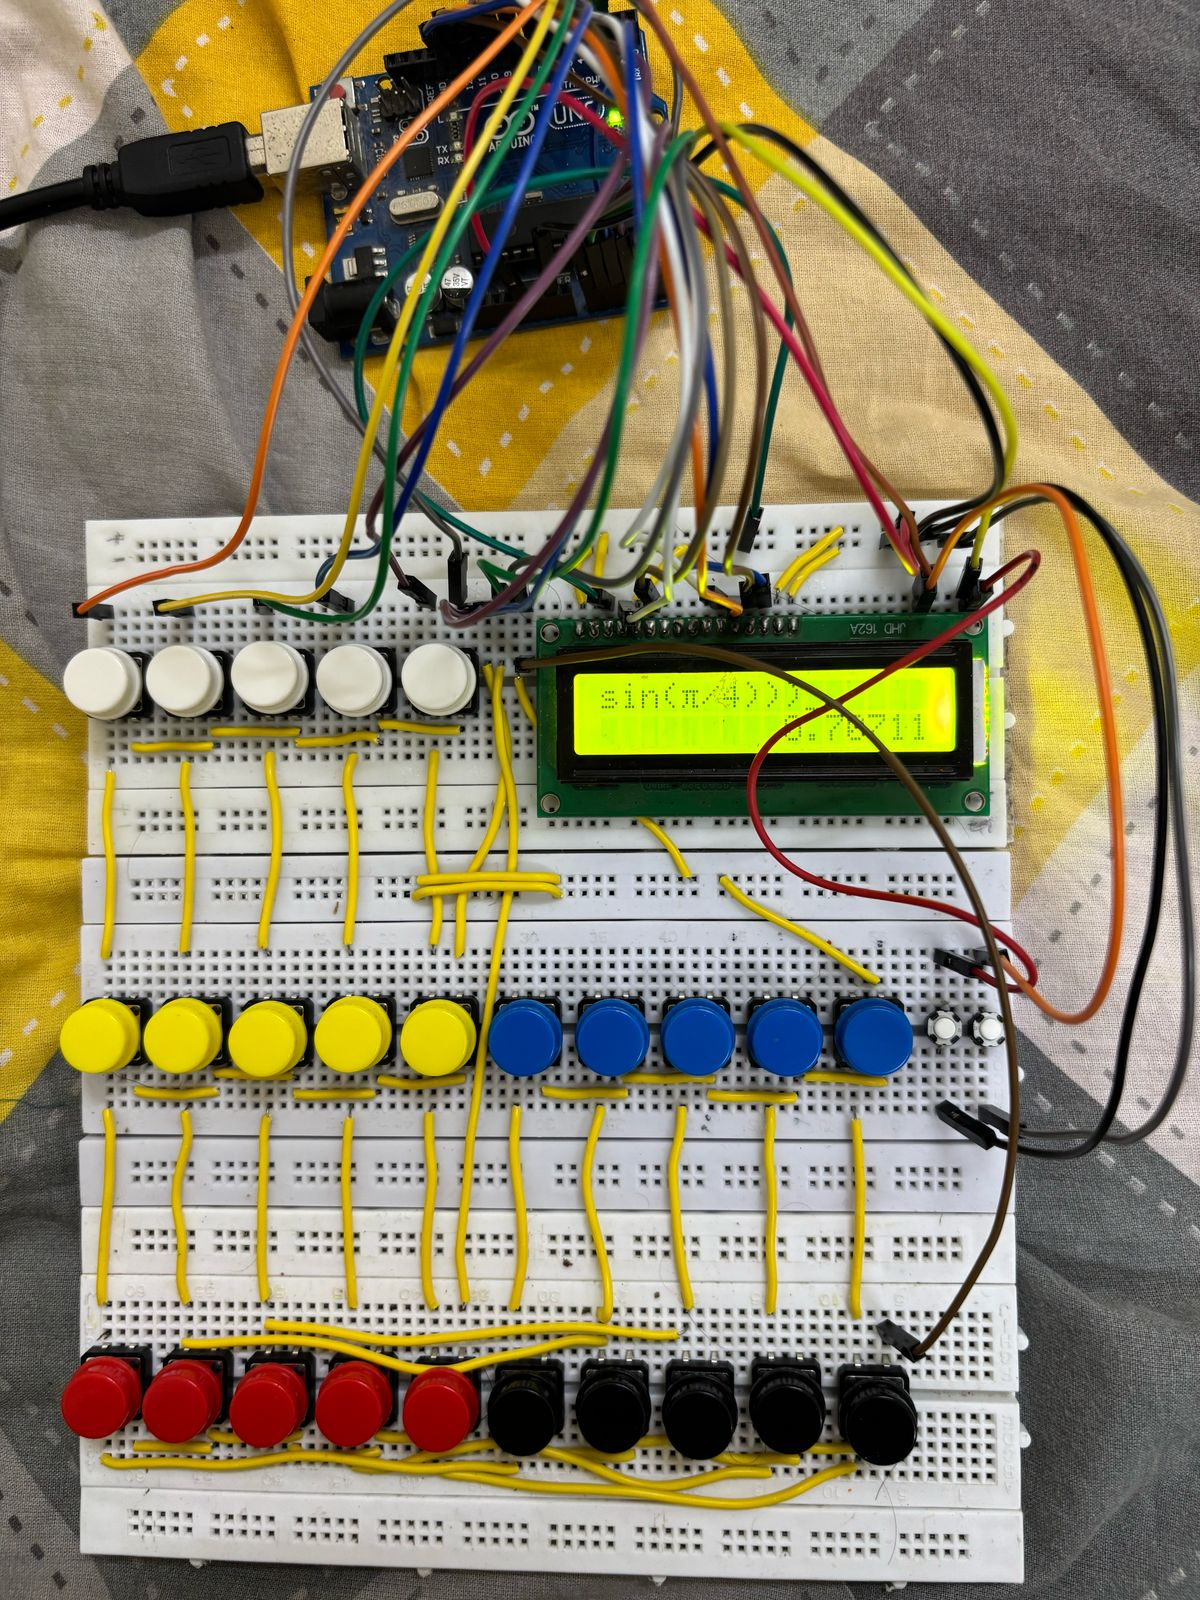
\includegraphics[width=0.5\textwidth]{figs/circuit.png}
  \end{center}
  \caption{}
  \label{fig:Circuit}
\end{figure}
\pagebreak
Code used may be found at, \url{https://github.com/ArjunPavanje/EE1003/blob/main/Hardware/Project/Calculator/main.c}
\section*{Overview}
\subsection*{Features}
The calculator supports:
\begin{itemize}
    \item Basic operations: addition $(+),$ subtraction $(-),$ multiplication $(*)$, division $(/),$ and exponentiation $($\textasciicircum$)$, factorial $(!)$.
    \item Trigonometric functions: $\sin$, $\cos$, $\tan$, $\arcsin$, $\arccos$, $\arctan$.
    \item Logarithmic functions: natural log ($\ln$), log base 10 ($\log_{10}$).
    \item Constants: $\pi$, $e$.
    \item Memory recall functionality.
    \item Autocompleting bracketis, movable cursor (to traverse code).
\end{itemize}
\subsection*{Hardware Overview}


The hardware consists of:
\begin{table}[H]
\centering
\begin{tabular}{|c|l|}
\hline
\textbf{Quantity} & \textbf{Component} \\
\hline
25 & Pushbuttons \\
\hline
1 & LCD 16 x 2 \\
\hline
1 & Arduino Uno\\
\hline
- & Wires \\
\hline
1 & Potentiometer \\
\hline
\end{tabular}
\caption{Materials Required}
\label{tab:materials}
\end{table}

\begin{itemize}
    \item A button matrix for user input.
    \item An Arduino Uno microcontroller (AtMega328p) to process inputs and execute calculations.
    \item Connecting a 16x2 LCD to arduino for displaying results.
    \item Connections between the button matrix, LCD, and Arduino Uno as shown in Figure~\ref{fig:circuit_schematic}.
\end{itemize}
The schematic for connections is as shown below,
\begin{figure}[H]
    \centering
    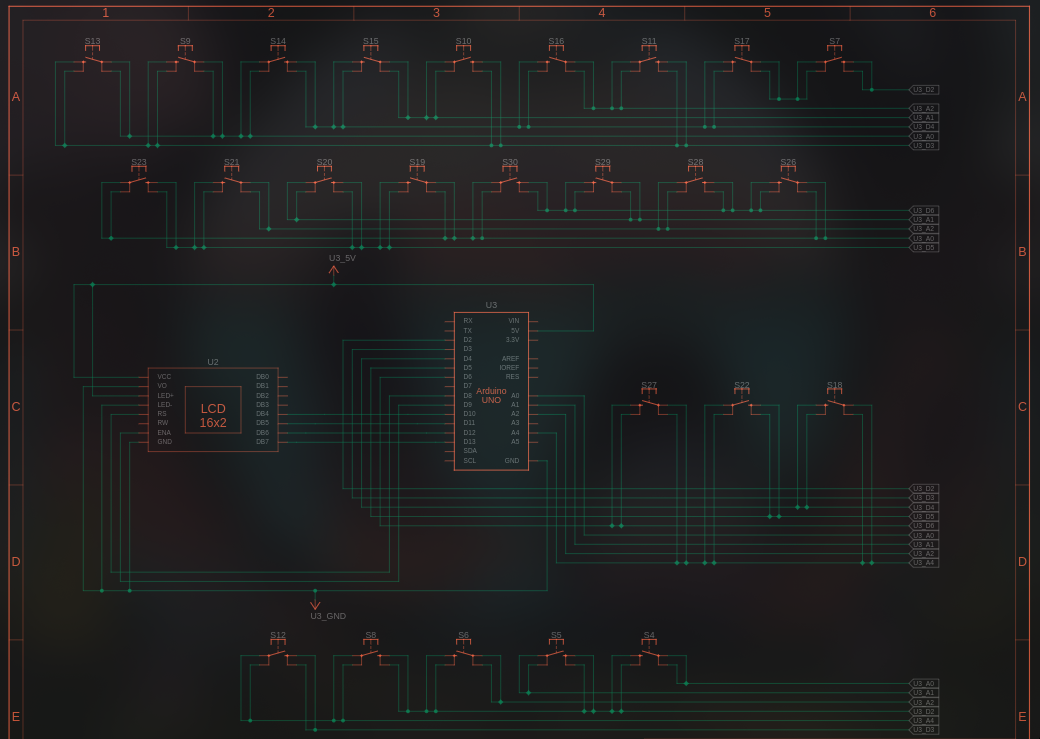
\includegraphics[width=\textwidth]{figs/circuit_schematic.png}
    \caption{Schematic of Circuit}
    \label{fig:circuit_schematic}
\end{figure}
\subsection*{Software Overview}
The software is implemented using avr-gcc. It includes:
\begin{itemize}
    \item Implementing button matrix to check which key is pressed.
    \item Storing input as a string (infix) 
    \item Converting infix to postfix using Shunting Yard algorithm.
    \item Evaluating postfix and returning answer.
    \item Support for functions like trigonometric functions (normal and inverse) logarithms, factorials, etc. All done without using \textbf{math.h} library, solving differential equations by RK4 method.
\end{itemize}
Now let us explore some of the features mentioned above in greater depth.
\section*{In Depth}
\subsection*{Button Matrix}
The button matrix is a grid of push-button switches arranged in rows and columns. It allows multiple buttons to be connected to the microcontroller using fewer pins. In my circuit, the rows are connected to analog pins (A0 to A4), while the columns are connected to digital pins (D2 to D6) of the Arduino.\newline
\textbf{Working Principle:}
\begin{itemize}
    \item The microcontroller scans the matrix by activating each row (setting it HIGH) one at a time while reading the columns for signals.
    \item When a button is pressed, it completes the circuit between its corresponding row and column.
    \item By identifying which row and column are active, the microcontroller determines which button was pressed.
    \item Suppose the first column is set to \( \text{HIGH} \), and a button (unknown to the circuit) is pressed. When reading from the rows, the microcontroller detects a signal from the second row. This confirms that the button pressed is the second button in the first column.
\end{itemize}
This idea helped us reduce the number of pins required to implement a calculator with $25$ buttons.
\begin{figure}[!ht]
\centering
\resizebox{1\textwidth}{!}{%
\begin{circuitikz}
\tikzstyle{every node}=[font=\large]
\draw (4.25,12) to[short] (4.25,6.25);
\draw (4.25,11.25) to[push button] (6.25,11.25);
\draw (4.25,10.25) to[push button] (6.25,10.25);
\draw (4.25,9) to[push button] (6.25,9);
\draw (4.25,7.75) to[push button] (6.25,7.75);
\draw (4.25,6.5) to[push button] (6.25,6.5);
\draw (7,12) to[short] (7,6.25);
\draw (7,11.25) to[push button] (9,11.25);
\draw (7,10.25) to[push button] (9,10.25);
\draw (7,9) to[push button] (9,9);
\draw (7,7.75) to[push button] (9,7.75);
\draw (7,6.5) to[push button] (9,6.5);
\draw (9.75,12) to[short] (9.75,6.25);
\draw (9.75,11.25) to[push button] (11.75,11.25);
\draw (9.75,10.25) to[push button] (11.75,10.25);
\draw (9.75,9) to[push button] (11.75,9);
\draw (9.75,7.75) to[push button] (11.75,7.75);
\draw (9.75,6.5) to[push button] (11.75,6.5);
\draw (12.5,12) to[short] (12.5,6.25);
\draw (12.5,11.25) to[push button] (14.5,11.25);
\draw (12.5,10.25) to[push button] (14.5,10.25);
\draw (12.5,9) to[push button] (14.5,9);
\draw (12.5,7.75) to[push button] (14.5,7.75);
\draw (12.5,6.5) to[push button] (14.5,6.5);
\draw (1.5,12) to[short] (1.5,6.25);
\draw (1.5,11.25) to[push button] (3.5,11.25);
\draw (1.5,10.25) to[push button] (3.5,10.25);
\draw (1.5,9) to[push button] (3.5,9);
\draw (1.5,7.75) to[push button] (3.5,7.75);
\draw (1.5,6.5) to[push button] (3.5,6.5);
\draw (6.25,12.5) to[short] (6.25,6.25);
\draw (6.25,13.5) to[short] (6.25,11.25);
\draw (3.5,12.75) to[short] (0.75,12.75);
\draw (6.25,13.5) to[short] (0.75,13.5);
\draw (11.75,15) to[short] (0.75,15);
\draw (0.75,14.25) to[short] (9,14.25);
\draw (9,14.25) to[short] (9,6.25);
\draw (14.5,15.75) to[short] (0.75,15.75);
\draw [ color={rgb,255:red,255; green,56; blue,56}, ](1.5,11.25) to[short] (0.75,11.25);
\draw [ color={rgb,255:red,240; green,51; blue,51}, ](1.5,10.25) to[short] (0.75,10.25);
\draw [ color={rgb,255:red,229; green,56; blue,56}, ](1.5,9) to[short] (0.75,9);
\draw [ color={rgb,255:red,246; green,49; blue,49}, ](1.5,7.75) to[short] (0.75,7.75);
\draw [ color={rgb,255:red,236; green,50; blue,50}, ](1.5,6.5) to[short] (0.75,6.5);
\node at (1.5,11.25) [circ] {};
\node at (1.5,10.25) [circ] {};
\node at (1.5,9) [circ] {};
\node at (1.5,7.75) [circ] {};
\node at (1.5,6.5) [circ] {};
\node at (3.5,11.25) [circ] {};
\node at (3.5,10.25) [circ] {};
\node at (3.5,9) [circ] {};
\node at (3.5,7.75) [circ] {};
\node at (3.5,6.5) [circ] {};
\node at (4.25,11.25) [circ] {};
\node at (4.25,10.25) [circ] {};
\node at (4.25,9) [circ] {};
\node at (4.25,7.75) [circ] {};
\node at (4.25,6.5) [circ] {};
\node at (6.25,6.5) [circ] {};
\node at (6.25,7.75) [circ] {};
\node at (6.25,9) [circ] {};
\node at (6.25,10.25) [circ] {};
\node at (6.25,11.25) [circ] {};
\node at (7,11.25) [circ] {};
\node at (7,10.25) [circ] {};
\node at (7,9) [circ] {};
\node at (7,7.75) [circ] {};
\node at (7,6.5) [circ] {};
\node at (9,11.25) [circ] {};
\node at (9,10.25) [circ] {};
\node at (9,9) [circ] {};
\node at (9,7.75) [circ] {};
\node at (9,6.5) [circ] {};
\node at (11.75,11.25) [circ] {};
\node at (9.75,11.25) [circ] {};
\node at (9.75,10.25) [circ] {};
\node at (9.75,9) [circ] {};
\node at (9.75,7.75) [circ] {};
\node at (9.75,6.5) [circ] {};
\node at (11.75,6.5) [circ] {};
\node at (11.75,7.75) [circ] {};
\node at (11.75,9) [circ] {};
\node at (11.75,10.25) [circ] {};
\node at (12.5,11.25) [circ] {};
\node at (12.5,10.25) [circ] {};
\node at (12.5,9) [circ] {};
\node at (12.5,7.75) [circ] {};
\node at (12.5,6.5) [circ] {};
\node at (14.5,6.5) [circ] {};
\node at (14.5,7.75) [circ] {};
\node at (14.5,9) [circ] {};
\node at (14.5,10.25) [circ] {};
\node at (14.5,11.25) [circ] {};
\draw [ color={rgb,255:red,255; green,51; blue,51}, ](1.75,11.25) to[short] (1.75,10.75);
\draw [ color={rgb,255:red,255; green,51; blue,51}, ](1.75,10.75) to[short] (13,10.75);
\draw [ color={rgb,255:red,221; green,44; blue,44}, ](13,11.25) to[short] (13,10.75);
\draw [ color={rgb,255:red,255; green,51; blue,51}, ](4.75,10.75) to[short] (4.75,11.25);
\draw [ color={rgb,255:red,255; green,51; blue,51}, ](7.5,10.75) to[short] (7.5,11.25);
\draw [ color={rgb,255:red,255; green,51; blue,51}, ](10.25,10.75) to[short] (10.25,11.25);
\draw [ color={rgb,255:red,255; green,51; blue,51}, ](1.75,10.25) to[short] (1.75,9.5);
\draw [ color={rgb,255:red,248; green,53; blue,53}, ](1.75,9.5) to[short] (13,9.5);
\draw [ color={rgb,255:red,255; green,51; blue,51}, ](13,9.5) to[short] (13,10.25);
\draw [ color={rgb,255:red,245; green,50; blue,50}, ](10.25,10.25) to[short] (10.25,9.5);
\draw [ color={rgb,255:red,233; green,47; blue,47}, ](7.5,10.25) to[short] (7.5,9.5);
\draw [ color={rgb,255:red,220; green,46; blue,46}, ](4.75,10.25) to[short] (4.75,9.5);
\draw [ color={rgb,255:red,251; green,50; blue,50}, ](1.75,9) to[short] (1.75,8.25);
\draw [ color={rgb,255:red,245; green,50; blue,50}, ](1.75,8.25) to[short] (13,8.25);
\draw [ color={rgb,255:red,238; green,58; blue,58}, ](13,9) to[short] (13,8.25);
\draw [ color={rgb,255:red,248; green,53; blue,53}, ](10.25,9) to[short] (10.25,8.25);
\draw [ color={rgb,255:red,253; green,53; blue,53}, ](7.5,9) to[short] (7.5,8.25);
\draw [ color={rgb,255:red,230; green,51; blue,51}, ](4.75,9) to[short] (4.75,8.25);
\draw [ color={rgb,255:red,255; green,51; blue,51}, ](1.75,7.75) to[short] (1.75,7);
\draw [ color={rgb,255:red,255; green,51; blue,51}, ](1.75,7) to[short] (13,7);
\draw [ color={rgb,255:red,234; green,57; blue,57}, ](13,7) to[short] (13,7.75);
\draw [ color={rgb,255:red,227; green,49; blue,49}, ](10.25,7.75) to[short] (10.25,7);
\draw [ color={rgb,255:red,240; green,56; blue,56}, ](7.5,7.75) to[short] (7.5,7);
\draw [ color={rgb,255:red,238; green,68; blue,68}, ](4.75,7.75) to[short] (4.75,7);
\draw [ color={rgb,255:red,255; green,51; blue,51}, ](1.75,6.5) to[short] (1.75,5.75);
\draw [ color={rgb,255:red,233; green,63; blue,63}, ](1.75,5.75) to[short] (13,5.75);
\draw [ color={rgb,255:red,229; green,56; blue,56}, ](13,6.5) to[short] (13,5.75);
\draw [ color={rgb,255:red,225; green,61; blue,61}, ](10.25,6.5) to[short] (10.25,5.75);
\draw [ color={rgb,255:red,236; green,65; blue,65}, ](7.5,6.5) to[short] (7.5,5.75);
\draw [ color={rgb,255:red,242; green,54; blue,54}, ](4.75,6.5) to[short] (4.75,5.75);
\node at (0.75,12.75) [circ] {};
\node at (0.75,13.5) [circ] {};
\node at (0.75,14.25) [circ] {};
\node at (0.75,15) [circ] {};
\node at (0.75,15.75) [circ] {};
\node at (0.75,11.25) [squarepole, color={rgb,255:red,236; green,65; blue,65}] {};
\node at (0.75,10.25) [squarepole, color={rgb,255:red,236; green,65; blue,65}] {};
\node at (0.75,9) [squarepole, color={rgb,255:red,236; green,65; blue,65}] {};
\node at (0.75,7.75) [squarepole, color={rgb,255:red,236; green,65; blue,65}] {};
\node at (0.75,6.5) [squarepole, color={rgb,255:red,236; green,65; blue,65}] {};
\node [font=\large] at (0,15.75) {$D2$};
\node [font=\large] at (0,15) {$D3$};
\node [font=\large] at (0,14.25) {$D4$};
\node [font=\large] at (0,13.5) {$D5$};
\node [font=\large] at (0,12.75) {$D6$};
\node [font=\large] at (0.25,11.25) {$A0$};
\node [font=\large] at (0.25,10.25) {$A1$};
\node [font=\large] at (0.25,9) {$A2$};
\node [font=\large] at (0.25,7.75) {$A3$};
\node [font=\large] at (0.25,6.5) {$A4$};
\draw (11.75,15) to[short] (11.75,6.25);
\draw (14.5,15.75) to[short] (14.5,6.25);
\draw (3.5,12.75) to[short] (3.5,6.25);
\end{circuitikz}
}%

\label{fig:my_label}
\end{figure}

\subsection*{Numerical Methods}
Key mathematical functions such as sine and logarithms are implemented using numerical methods like Runge-Kutta (RK4).

In this section, we discuss the application of the Runge-Kutta 4th order (RK4) method for solving differential equations. The RK4 method is a powerful and widely used technique to approximate solutions to ordinary differential equations (ODEs). Below, we list the differential equations used for various functions solved using the RK4 method.

\subsubsection*{Runge-Kutta 4th Order (RK4) Method}

The RK4 method is given by the following iterative steps to solve the differential equation \( \frac{dy}{dx} = f(x, y) \):
\[
k_1 = h f(x_n, y_n)
\]
\[
k_2 = h f\left( x_n + \frac{h}{2}, y_n + \frac{k_1}{2} \right)
\]
\[
k_3 = h f\left( x_n + \frac{h}{2}, y_n + \frac{k_2}{2} \right)
\]
\[
k_4 = h f(x_n + h, y_n + k_3)
\]
\[
y_{n+1} = y_n + \frac{1}{6} \left( k_1 + 2k_2 + 2k_3 + k_4 \right)
\]
where \( h \) is the step size, \( y_n \) is the value of the solution at time \( x_n \), and \( f(x, y) \) represents the differential equation.

\subsubsection*{Trigonometric Functions}

For trigonometric functions, we solve the following differential equation whose solution is \( y(x) = \sin(x) \):
\[
\frac{d^2y}{dx} + y = 0;
\]
 Once we have the function to calculate sine, we can use the following facts to calculate cosine and tan. 
\begin{align*} 
 \cos(x) &= \sin \left( \frac{\pi}{2} - x \right)\\ 
 \tan(x) &= \frac{\sin(x)}{\cos(x)}
\end{align*}

\subsubsection*{Inverse Trigonometric Functions}

For inverse trigonometric functions, we solve the differential equation whose solution is \( y(x) = \arcsin(x) \):
\[
\frac{dy}{dx} = \frac{1}{\sqrt{1 - x^2}}
\]
Once we obtain the method to calculate inverse sine, cosine inverse can be implemented by using the property, 
\begin{align*}
    \arccos(x) + \arcsin(x) = \frac{\pi}{2}
\end{align*}
to obtain tan inverse we need to solve a seperate differential equation,
\begin{align*}
    \frac{dy}{dx} = \frac{1}{1+x^2}
\end{align*}
\begin{figure}
  \begin{center}
    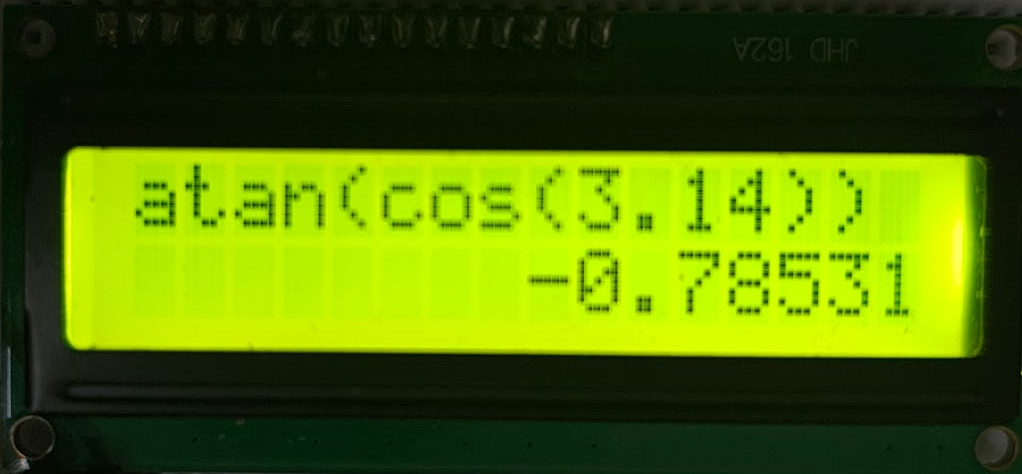
\includegraphics[width=0.95\textwidth]{figs/trig.png}
  \end{center}
  \caption{Trigonometric and Inverse Trigonometric Functions}\label{fig:Trigonometric and Inverse Trigonometric Functions}
\end{figure}

\subsubsection*{Logarithmic Function}

For the logarithmic function, we solve the differential equation whose solution is \( y(t) = \ln(t) \):
\[
\frac{dy}{dx} = \frac{1}{x}
\]
\begin{figure}[h!]
  \begin{center}
    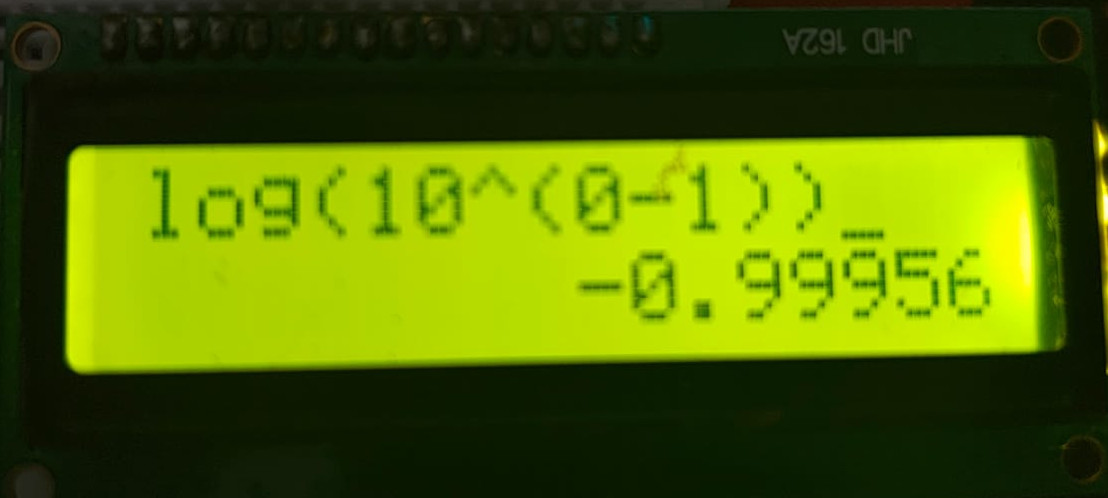
\includegraphics[width=0.7\textwidth]{figs/ln.png}
  \end{center}
  \caption{Logarithm (Base 10)}\label{fig:Log base 10}
\end{figure}

\subsubsection*{Power (Exponent) Function}

For the power function, we solve the differential equation whose solution is $y = x^a$:
\[
\frac{dy}{dx} = \frac{ay}{x}
\]

% \section{Showcase of functions implemented}
% \subsection{BODMAS}
% \begin{figure}[H]
%     \centering
%     \includegraphics[width=0.5\linewidth]{}
%     \caption{BODMAS}
% \end{figure}

\begin{figure}
  \begin{center}
    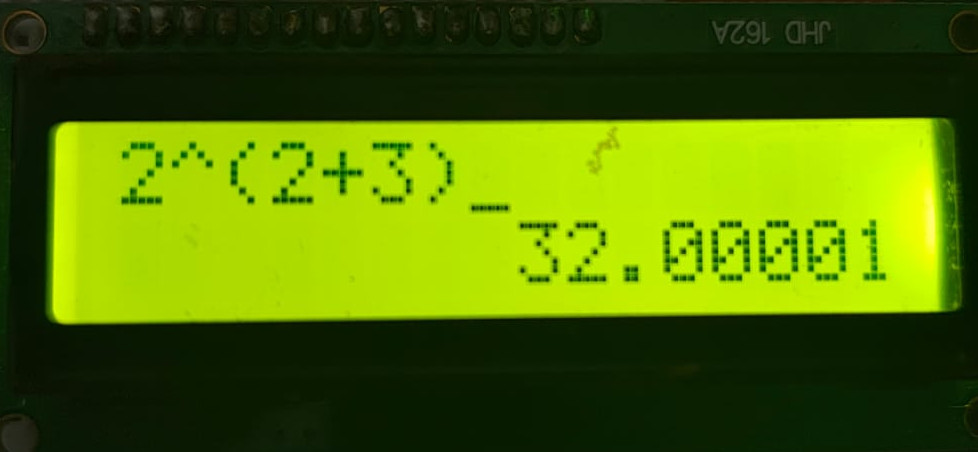
\includegraphics[width=0.8\textwidth]{figs/pow.png}
  \end{center}
  \caption{Power}
  \label{fig:Power}
\end{figure}
\begin{figure}
  \begin{center}
    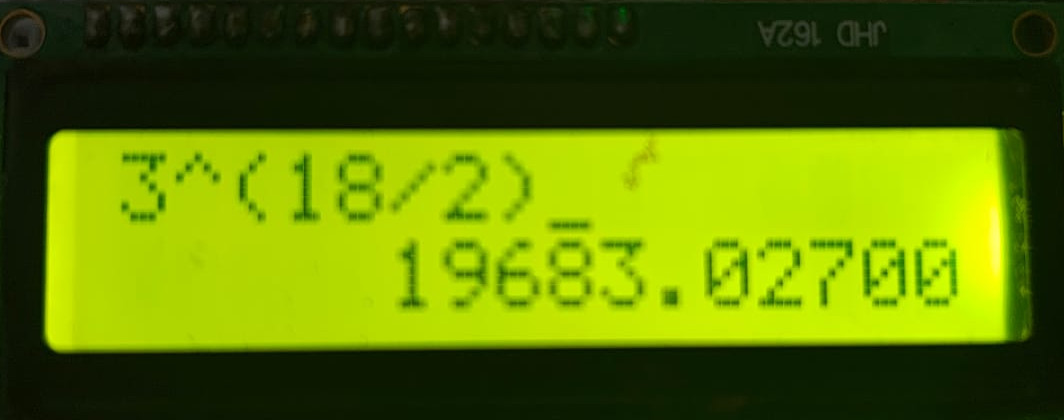
\includegraphics[width=0.8\textwidth]{figs/pow1.png}
  \end{center}
  \caption{Exponent}
  \label{fig:Exponent}
\end{figure}
\begin{figure}
  \begin{center}
    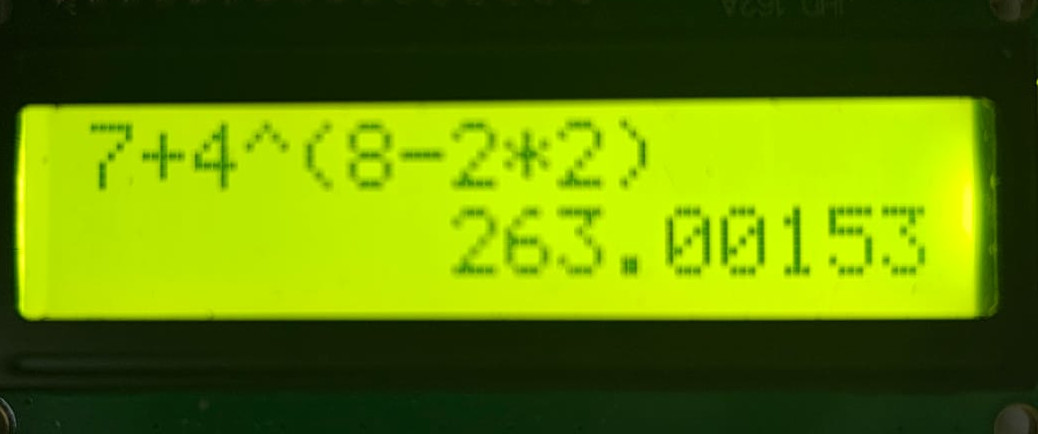
\includegraphics[width=0.8\textwidth]{figs/bod.png}
  \end{center}
  \caption{Bodmas}
  \label{fig:Bodmas}
\end{figure}
\section*{Conclusion}
This project has demonstrated my attempt to implementation of a fully functional calculator using a button matrix and AtMega328p microcontroller (arduino uno) implemented using avr-gcc and differential equations. 

\end{document}
